\documentclass{beamer}

\title[Pipelined FFT]{A Pipelined FFT Implementation in Verilog}
\author{Saji Champlin}
\institute{University of Minnesota}
\date{\today}
\subtitle{EE5327 Project Presentation}
\usetheme[secheader]{Boadilla}
\useinnertheme{rectangles}
\usefonttheme{professionalfonts}
\beamertemplatenavigationsymbolsempty


\usepackage{amsmath}
% \usepackage[margin=1in]{geometry}
\usepackage[english]{babel}
% \usepackage[shortlabels]{enumitem}
% \usepackage[group-separator={,}]{siunitx}
\usepackage{multicol}
\usepackage{caption}
\usepackage{pdfpages}
\usepackage[outputdir=build]{minted}
\usepackage{tikz}
\usepackage{wrapfig}
\usepackage{graphicx}
\usepackage{listings}
% \usepackage{biblatex}
% \addbibresource{refs.bib}
\graphicspath{ {./figures/} }
\usetikzlibrary{patterns}

% minted should always be footnotesize and single spaced.
\setminted{fontsize=\footnotesize,baselinestretch=1, frame=lines, breaklines}

% Don't print section numbers
% \setcounter{secnumdepth}{0}
%
% % disable indentation for new paragraphs.
% \setlength{\parindent}{0pt}
% \setlength{\parskip}{0pt plus 0.5ex}


\begin{document}

\frame{\titlepage}

\section{Overview}

\begin{frame}
	\frametitle{What is an FFT?}

	An FFT is a very efficient way of computing the DFT of a given sequence of values.

	A naive DFT is $O(N^2)$, whereas an FFT is $O(N \log{N})$. This is massive at high
	values of $N$.

\end{frame}

\begin{frame}
	\frametitle{What is a Pipelined FFT?}
	A pipelined FFT is similar to a pipelined CPU:
	\begin{columns}
		\column{0.38\linewidth}
		\begin{enumerate}
			\item Execution is split into "Stages"
			\pause
			\item Each stage is connected by registers
			\pause
			\item Executing a stage takes 1 cycle
		\end{enumerate}
		\column{0.58\linewidth}
		\onslide
		\centering
		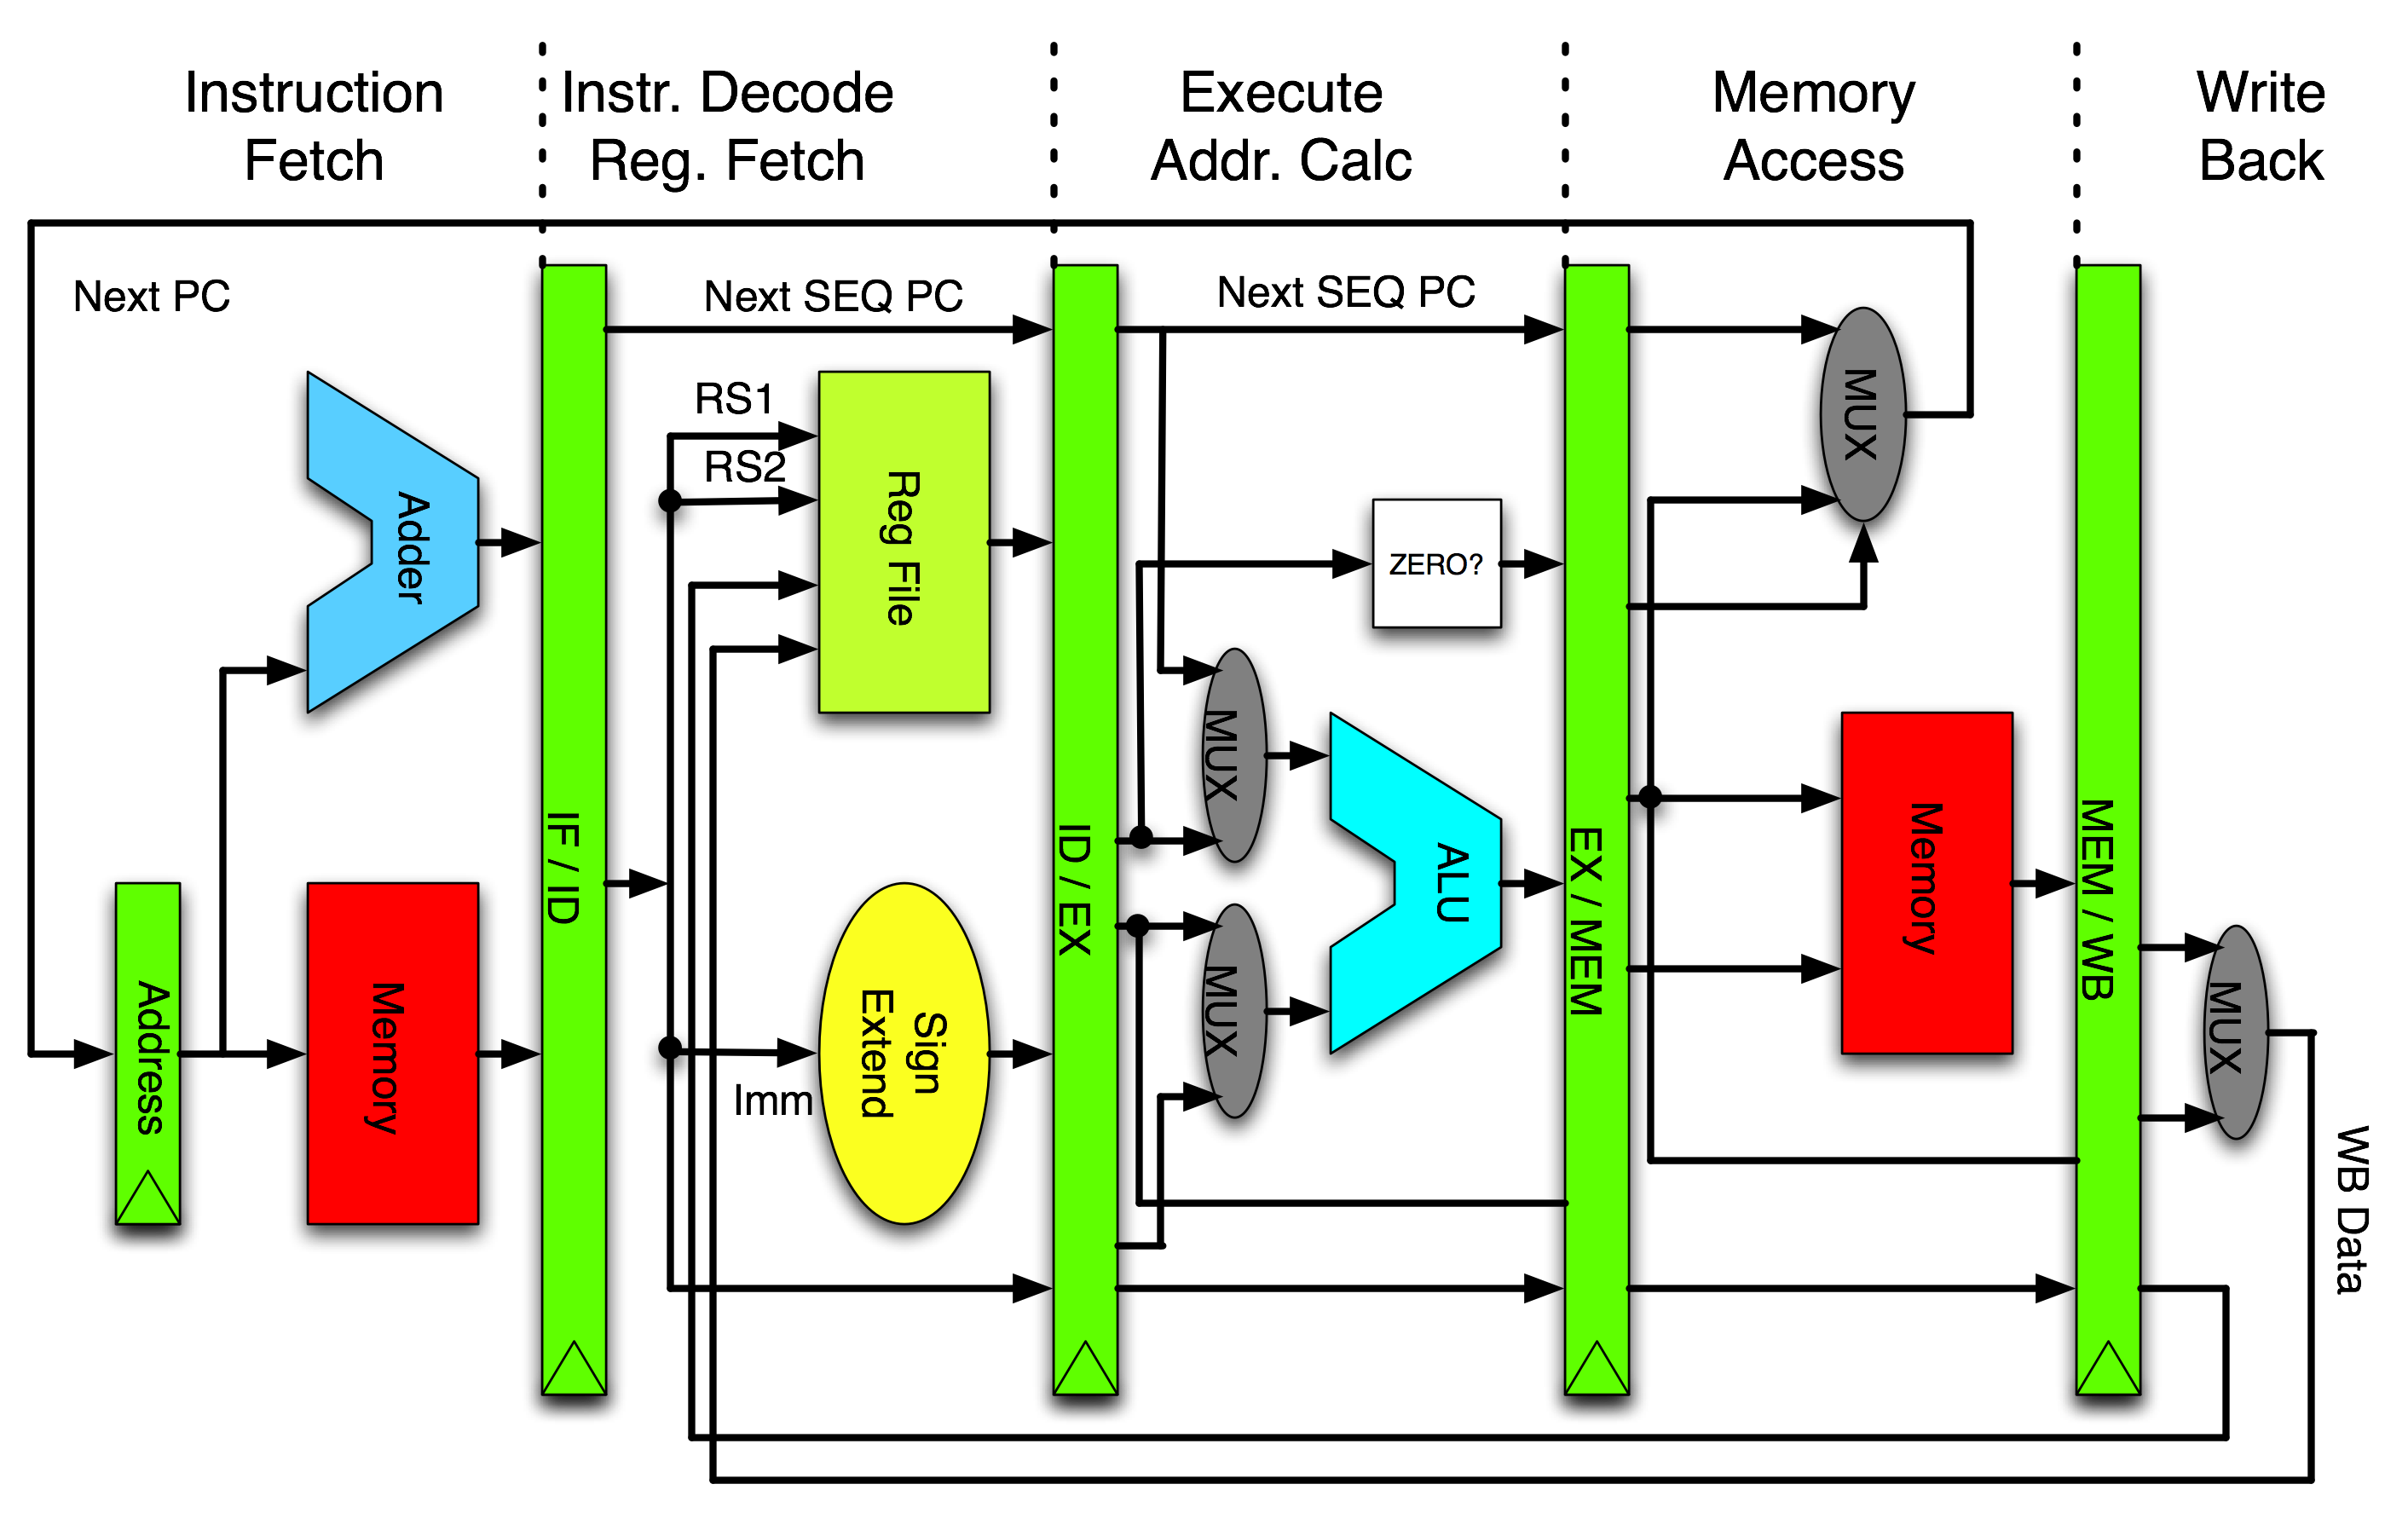
\includegraphics[width=\linewidth]{Pipeline_MIPS.png}
		\captionof{figure}{MIPS pipeline example.}
	\end{columns}

\end{frame}


\begin{frame}
	\frametitle{How does this work in an FFT?}
	FFTs have $P$ layers where $2^P = N$, so we simply insert registers
	each layer and ensure that a layer can run in a single clock cycle
	\footnote{Single clock isn't a strict requirement, but it does simplify design}.
	\begin{figure}
		\centering
		\begin{tikzpicture}
			\foreach \x in {0,...,3} {
				\draw (0,-\x) node[rectangle,left,draw] (l0_\x) {$x[\x]$};
				\node[circle, draw, minimum size=0.2mm] (l1_\x) at (1,-\x) {}; 
				\node[circle, draw, minimum size=0.2mm] (l2_\x) at (3,-\x) {}; 
				\node[circle, draw, minimum size=0.2mm] (l3_\x) at (5,-\x) {}; 
				\draw [-latex](l0_\x) -- (l1_\x);
				\draw [-latex](l1_\x) -- (l2_\x);
				\draw [-latex](l2_\x) -- (l3_\x);
				\draw [-latex](l3_\x) -- ++(1,0) node[rectangle, right, draw] {$X[\x]$}; 
			}
			
			\draw [-latex](l1_0) -- (l2_1);
			\draw [-latex](l1_1) -- (l2_0);
			\draw [-latex](l1_2) -- (l2_3);
			\draw [-latex](l1_3) -- (l2_2);

			\draw [-latex](l2_0) -- (l3_2);
			\draw [-latex](l2_1) -- (l3_3);
			\draw [-latex](l2_2) -- (l3_0);
			\draw [-latex](l2_3) -- (l3_1);

			\draw [latex-](l2_3) -- ++(0,-1) node[rectangle, below,draw=orange!30] (hi) {registers};
			
			\draw [-latex](hi) -| (l1_3);
			\draw [-latex](hi) -| (l3_3);

			
		\end{tikzpicture}
		\caption{Example FFT structure where $N=4$.}
	\end{figure}
\end{frame}

\section{Design}

\subsection{Architecture}

\begin{frame}
	\frametitle{General structure}
	An FFT is an arrangement of "Butterfly" transforms and twiddle factors.
	A butterfly transform is a radix-2 DFT with a complex multiplication factor.
	\begin{align*}
		y_0 &= x_0 + x_1 w_n^k \\
		y_1 &= x_0 - x_1 w_n^k
	\end{align*}
	\begin{figure}
		\centering
		\begin{tikzpicture}
			\node [left](x0) at (0,0) {$x_0$};
			\node [left](x1) at (0,-1) {$x_1$};
			\node [right](y0) at (1.5, 0) {$y_0$};
			\node [right](y1) at (1.5, -1) {$y_1$};

			\draw [blue](x0) -- (y0);
			\draw [blue](x0) -- (y1);

			\draw [red](x1) -- (y0);
			\draw [red](x1) -- (y1);

		\end{tikzpicture}
	\end{figure}
	The twiddle factor $w$ is used to rotate the values by a given amount depending on the
	portion of the FFT being calculated. $w_n^k = e^{-2\pi i k / n}$.
\end{frame}

\subsection{Complex Multiplier}
\begin{frame}
	\frametitle{Complex Multiplier}
	This is a primitive we use in the butterfly module later. It is tricky due
	to being fixed-point and signed. \pause Recall that for complex numbers $z$ and $y$,
	their product is
	\begin{align*}
		z y = (ac + bd) + (ad + bc)i
	\end{align*}
	\pause
	We need fixed point math to store $w$ values. Fixed point multiplication doubles
	the binary point (Q2.14 becomes Q4.28) so we must also account for this in the multiplier.

\end{frame}


\begin{frame}[fragile]
	\frametitle{Complex Multiplier, Cont.}
	The crux of the code is as follows (\texttt{WIDTH} and \texttt{FIXED\_POINT} are parameters):
\begin{minted}{verilog}
reg signed [2*WIDTH - 1:0] res_re, res_im;
// the shifted 1 by fixed point -1 is for rounding.
localparam ROUND_FACTOR = 1 << (FIXED_POINT -1);
assign y0_re = res_re[FIXED_POINT + WIDTH-1:FIXED_POINT];
assign y0_im = res_im[FIXED_POINT + WIDTH-1:FIXED_POINT];
always @(posedge clk) begin
  res_re <= a_re * b_re - a_im * b_im + ROUND_FACTOR;
  res_im <= a_re * b_im + a_im * b_re + ROUND_FACTOR;
end
\end{minted}
The round factor is used to improve precision when truncating.
\end{frame}

\subsection{Butterfly}
\begin{frame}[fragile]
	\frametitle{Butterfly transform}
	Comparatively, the butterfly is simpler, because addition/subtraction does not require
	special behavior for fixed-point math.
\begin{minted}{verilog}
cplx_mul #(.WIDTH(WIDTH)) twiddle_mul (clk, b_re, b_im, twiddle_re, twiddle_im, product_re, product_im);
always @(*) begin
  y0_re = a_re + product_re;
  y0_im = a_im + product_im;
  y1_re = a_re - product_re;
  y1_im = a_im - product_im;
end
\end{minted}
\begin{block}{Note}
I use a combinational always block to prevent needing two clocks to get a result.
\end{block}
\end{frame}

\section{Verification}

\subsection{Simulation \& Testbench}
\begin{frame}[fragile]
	\frametitle{Simulation Overview}
	Complex number arithmetic is challenging to do in Verilog, is there a better way
	to check for correctness?

	\pause
	\structure{Yes!} We can use a tool called \texttt{cocotb} to generate stimulus and
	test module behavior for correct output in Python.

	\pause
\begin{minted}{python}
@cocotb.test()
async def test_cplx(dut):
    cocotb.start_soon(Clock(dut.clk, 1, 'ns').start())

    await set_terms(dut, 2 + 1j, 3 + 4j)
    await RisingEdge(dut.clk)
    await ReadWrite()
    res = await get_product(dut)
    assert res == 2 + 11j
\end{minted}
\captionof{lstlisting}{Simple \texttt{cocotb} test for the complex multiplier}
\end{frame}

\begin{frame}[fragile]
	\frametitle{Cocotb Details}
	\begin{itemize}
\item This test is simple, but supported by helper functions
	that convert python types to inputs for the DUT.
\item t can use multiple simulator backends, including Synopsys VCS,
	as well as open-source software like Verilator or Icarus Verilog.

\item	Because we use floating point in Python, we need to allow for some tolerance
	when comparing with fixed-point values from the DUT:
\begin{minted}{Python}
    res = await get_product(dut)
    expected = n1 * n2
    assert math.isclose(res.real,expected.real, abs_tol=0.00390625)
    assert math.isclose(res.imag,expected.imag, abs_tol=0.00390625)
\end{minted}

\item A significant advantage with \texttt{cocotb} is easy randomized tests.


\end{itemize}

\end{frame}

\begin{frame}[fragile]

The output of cocotb for a test suite is as follows:
\begin{minted}{c}
******************************************************************
** TEST                                  STATUS  SIM TIME (ns)  **
******************************************************************
** tests.test_cplx_mul.test_unity         PASS           1.00   **
** tests.test_cplx_mul.test_negation      PASS           1.00   **
** tests.test_cplx_mul.test_imag          PASS           1.00   **
** tests.test_cplx_mul.test_cplx          PASS           1.00   **
** tests.test_cplx_mul.test_rand_ints     PASS         100.00   **
** tests.test_cplx_mul.test_rand_floats   PASS        1000.00   **
******************************************************************
** TESTS=6 PASS=6 FAIL=0 SKIP=0                       1104.01   **
******************************************************************
\end{minted}

\begin{block}{Remark}
	The latter tests use randomly generated complex numbers from Python, in a range where overflow
	will not occur.
\end{block}
\end{frame}


\begin{frame}
	\frametitle{Sidenote: Should you use \texttt{cocotb}?}
	\structure{You should use \texttt{cocotb} iff:}
	\begin{enumerate}
		\item The inputs and outputs of your modules are non-trivial (fixed-point, complex, etc)
		\item Performing the correct operation in Python is easy (complex multiplication)
		\item A Verilog testbench would use the same operations of your DUT.
	\end{enumerate}
	\structure{You \emph{shouldn't} use \texttt{cocotb} if:}

	\begin{enumerate}
		\item You already have working Verilog testbenches.
		\item Your DUT is not easy to replicate in Python.
	\end{enumerate}

\end{frame}

\begin{frame}
	\frametitle{Waveforms}
\end{frame}

\section{Summary}

\end{document}
